\documentclass[a4paper,6pt]{article}
\usepackage[utf8]{inputenc}
\usepackage{graphicx}
\usepackage{url}
\usepackage{amssymb}
\bibliographystyle{unsrt}
\usepackage{listings}
%\usepackage{fullpage}
\usepackage[bookmarks]{hyperref}

\usepackage[section]{minted}

\title{
  \begin{center}
    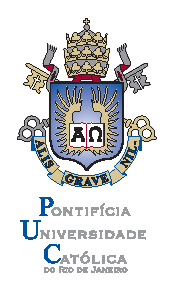
\includegraphics[width=200pt]{graphics_tables/bras_vert_cor.eps}
  \end{center}
  \begin{center}
  \end{center}
   Research Design and Academic Writing 2012.2\\
  \textit{Runtime introspection for C++11}
}

\author{Maximilien de Bayser}

\begin{document}

\maketitle
\newpage

\begin{abstract}
Many object-oriented languages support some kind of runtime introspection that allows programmers to
navigate through meta-data describing the available classes, their attributes and methods. In general,
the meta-data can be used to instantiate new objects, manipulate their attributes and call their methods.
The meta-programming enabled by this kind of reflection has proven itself useful in a variety of applications
such as object-relational mappings and inversion-of-control containers and test automation

Motivated by the need of programmatic support for composition and configuration of software components
at runtime, in this work we show how to implement a runtime reflection support for \texttt{C++11}, using the available
runtime type information, template metaprogramming and source code analysis. We will show the capabilities
of the reflection \texttt{API} and the memory footprint for different kinds of meta-data.
The API relies on a few features introduced by C++11, the new ISO standard for C++.
Our reflection system is not invasive as it requires no modifications whatsoever of the application code. 
\end{abstract}


\section{Introduction}

% TODO: talvez seja uma boa usar as definicoes e termos do Lakos da secao 5.4

Every computational system is built to solve a particular problem. As a consequence, all data structures and procedures
of a program represent this particular problem domain. A reflective system is one that is augmented with a representation
of itself. In other words, a reflective program can perform computations about its own computation.

Self-reference is a deeply philosophical issue and is often identified as an essential property of intelligence. For instance,
in his highly influential book, \texttt{Gödel, Escher, Bach: An Eternal Golden Braid}, Hofstadter \cite{Hofstadter} discusses how
Gödel's incompleteness theorem, biological systems and human intelligence all exhibit forms of self-reference and
self-representation. As a result, it should come as no surprise that the first studies of computational reflection came
from the mathematical logic and artificial intelligence communities.

One of the earliest works in computational reflection was Smith's \texttt{3-LISP} language \cite{Smith}, which he proposed as a first step towards
intelligent systems that could reason about themselves. Smith first considered the possibility of a self-referential language
when he wrote an interpreter for the KRL language in that same language. Later he refined his ideas in a new version of the
LISP language where the interpreter would expose details about the interpretation to the program being interpreted. In this language,
which he called \texttt{3-LISP}, an interpreted program could manipulate its own expressions, continuations and environments, thereby
changing its own behavior.

One aspect of self-reference is that it can go on indefinitely. An interpreter written in the same reflective language that it
interprets opens up the possibility of infinite levels of reflection, requiring what Smith called an infinite tower of interpreters.
In practice, this issue is solved by a so-called meta-circular interpreter that is able to simulate the infinite levels of regression.

Smith also outlined six general properties of reflective systems. The first principle is the requirement of a causal connection between
its self-representation and its behavior. This means that a reflective program should use this information to alter its
behavior. It would be useless if a process only contemplated itself without any further consequence. The second property is that
self-reference is necessarily associated to a theory, a representation of the knowledge, of itself. The third property is that
self-reference does not entail the ability of focusing on its current self. A process can only inspect what it was doing before
taking up the reflective activity. Otherwise, it could reflect about itself reflecting about itself reflecting ... and so on.
The fourth property of reflection is that it enables a finer grained control over the behavior of a program. In other words, it
enables more sophisticated programming techniques. The fifth property is that total detachment or objectivity is not possible,
because the self-knowledge is represented in the same formalism. The last property is that ``..Being reflective is a stronger
requirement on a calculus than simply being able to model the calculus in the calculus''. The ability to reflect cannot be
programmed from the inside. A Turing machine can simulate another Turing machine augmented with reflective capabilities but it
cannot reflect about itself. We will return to some of these points throughout this discussion.

The next step in the research of computational reflection was its application to object-oriented languages. In her seminal paper, Maes \cite{Maes}
outlined the basic features of reflection in an object-oriented context. The language \texttt{3-KRS}, built to demonstrate her ideas, had the
following properties:

\begin{enumerate}
 \item A split between object-level and meta-level. The meta-level was comprised of objects containing informations about the user-defined
object.
 \item A uniform self representation: everything in \texttt{3-KRS} is an object and consequently has a meta-object that can be inspected.
 \item A complete self-representation. Every object has a meta-object.
 \item Self-consistency. The meta-level is consistent with the object level and \emph{vice versa}. A modification to one entails a modification
to the other. 
  \item Modifiable self-representation. Meta-objects in \texttt{3-KRS} can be modified.
\end{enumerate}

This design has several interesting consequences. First of all, properties 2 and 3 guarantee that all entities in a program can be
inspected by the program itself. This alone opens up a myriad of possibilities of generic programming, auditing and debugging.
Second, properties 4 and 5 enable the modification of object properties at runtime since, to maintain consistency, modifications
in the meta-level must be reflected in the object level. Third, as a consequence of the uniformity property, the meta-objects themselves
have meta-objects that can be modified. An example of a modification is the addition, removal or redefinition of methods and attributes.

The same design was followed in the implementation of the Common Lisp Object System (CLOS) and its Meta Object Protocol (\texttt{MOP}) \cite{Kiczales}.
The idea behind CLOS, according to the authors, was to define a region in the design-space of programming languages instead of
a point. Because there are several ways to implement object-oriented mechanisms, each involving different trade-offs, CLOS was
designed to be adaptable to the needs of different application domains. To enable this, some basic mechanisms such as the
rules of method calls could be modified by specializing meta-classes.

Sadly, all this flexibility also introduces several new problems. One is that of meta-stability. In the words of Kiczales and colleagues,
the modification of objects at runtime could result in spectacular failure modes \cite{Kiczales}. Another serious issue is the performance price
that inevitably must be paid to compensate for the added flexibility. Taking this into account, the design of the \texttt{MOP} restricts
the possibilities of modifications in critical mechanisms, such as method dispatch to enable implementers to make optimizations.
For example, there are methods of meta-classes that are required to be idempotent. This allows the implementation to call
these methods only once and \emph{memoize} the result. However, even with these considerations there is anecdotal evidence
that suggests that opening the language for modification results in a performance overhead that is prohibitive for some applications \cite{Lee}.

Another problem is the runtime infra-structure needed for a self-modifiable program. So far in this discussion, it was implicit
that all discussed languages were interpreted rather than compiled. Even considering that everything is ultimately interpreted
by the underlying hardware, it would be a considerable challenge to implement the previously discussed kind of dynamism in
a compiled language. The language runtime would have to include a compiler. There are tools that can be used to provide
a meta-object protocol for compiled languages, but they are restricted to compilation or load time \cite{Chiba95} \cite{Chiba2000}.

Of course it is difficult to draw a line between compiled and interpreted languages. One reason, as mentioned, is that the hardware
itself is an interpreter. Another one is that, even interpreted languages, are usually parsed and compiled to a representation that is
easier to handle by the interpreter. A criteria that we can adopt is the following: in compiled languages, the interpreter, be it hardware
or software, cannot understand the source language, while in interpreted languages it does. This property of interpreted
languages is often made explicit by the presence of an \texttt{eval} primitive that can be called by the program at runtime
to interpret more code in the form of source text.

A further issue is that runtime modification of a program would be difficult to conciliate with static typing, which is the norm
in compiled languages. In languages with static typing, types are used as contracts between different parts of a program. 
These contracts enable the compiler to generate optimal code for method invocations because it knows precisely what argument
types to expect.

For the reasons mentioned above, reflection in compiled languages, if supported, is usually restricted to what is known
as introspection. This means that the meta-data can be inspected but not modified, what implies that no changes
have to be reflected back to the object level. However, somewhat ironically, in statically typed languages, this
limited form of reflection is much more useful than it would be in dynamic languages, because it enables the use of types
that were unknown at compile time. In other words, introspection can be used to simulate dynamic typing in a statically typed language.

The primary example of a statically typed language with native introspection is \texttt{Java}, so we will discuss its reflective features in detail
and use it as an inspiration for the implementation of an introspection support for \texttt{C++}. Finally, we wish to point out that reflection
is not an exclusive property of the programming language. Reflection is also possible at other abstraction layers, such as the architectural
level.


\section{Introspection in Java}

\texttt{Java} is a statically typed language that is compiled to the bytecode of the \texttt{Java} Virtual Machine (\texttt{JVM}). The fact that it is not executed
directly by hardware does not mean that it can be seen as an interpreted language: there is no \textbf{eval} primitive.
The reason for analyzing \texttt{Java} in detail in this discussion is that \texttt{Java} has a native introspection support and has many
similarities with \texttt{C++}.

Each source file of \texttt{Java} contains the definition of a single class and is compiled to a bytecode file called a class file.
Class files have a dual role in \texttt{Java}. The first role corresponds to that of header files in \texttt{C++}: the
declaration of types and methods used by other compilation units. The second second role corresponds roughly to that of
\texttt{C++} object files, containing data to direct the linkage of compilation units. This dual use forces this file format to
preserve information about classes, such as the the number and signature of methods, attributes and constructors.
Furthermore, compilation units in \texttt{Java} are linked at runtime when they are loaded into the \texttt{JVM}. Given that
class meta-data is present when classes are loaded, it is only logical to make it available to the programmer by means
of an introspection API instead of discarding it after linking. Another interesting feature of \texttt{Java} is that the loading
of classes can be customized. Application programmers can provide their own custom class loaders, which presents the
opportunity to modify classes before they are linked, enabling a meta-object protocol at load time \cite{Chiba2000}.

Having seen how class meta-data is obtained by the \texttt{JVM}, let us now turn our attention to the architecture of the
introspection \texttt{API}. In \texttt{Java}, every class is associated to a meta-object of the class \texttt{java.lang.Class} and every object
inherits from the base class \texttt{java.lang.Object}. The \texttt{Object} base class can be used to obtain a reference to the meta-object of
its class. Only single inheritance of implementation is possible in \texttt{Java} so this reference always points unambiguously to the
meta-object of the most concrete class of an object. Observe that, because in \texttt{Java} classes are not first-class citizens, they
cannot be collapsed with their meta-objects as is the case in prototype-based object-oriented languages.

The class \texttt{java.lang.Class} has class-global methods to search classes by name and to list all classes, so the meta-data for all
classes is reachable at runtime. The information made available by an instance of \texttt{java.lang.Class} basically consists of the
class's visibility, a list of its constructors, a list of its attributes and a list of its methods. These lists include not only
\texttt{public} entities but also those with \texttt{protected}, \texttt{private} or \texttt{package} visibility, making it
possible to bypass the access restrictions.

The entities accessible through a class meta-object are meta-objects as well. Attribute meta-objects are instances of the class
\texttt{java.lang.reflect.Field}, constructors and methods are represented by the classes \texttt{java.lang.reflect.Constructor} and \texttt{java.lang.reflect.Method}
respectively. There is no need to go into much detail here so we will only present a brief summary of the functionality provided
by theses classes.

The \texttt{Field} meta-object can be used to inspect the name and the type of an attribute. The type information is given in the form of
a reference to a Class meta-object. In addition, this object can be used to obtain and to change the value of the given attribute in
a specific object. The value is returned using a reference to the universal base class, \texttt{Object}. A minor difficulty arises due to the
fact that primitive types are not objects in \texttt{Java}. To deal with this, for each primitive type \texttt{Java} defines a container class such
as \texttt{java.lang.Integer} and seamlessly performs \emph{auto-boxing} when necessary.

Constructor meta-objects provide information about the number of arguments in addition to the type of each one of them. Constructor
objects also have a method that takes an array of Objects calls the reified constructor passing these arguments, and returns a new
instance of the class this meta-object is associated with. The class meta-object has a shortcut method called \texttt{newInstance}
that finds a constructor based on the types of its arguments and uses it to return a new object.

Finally, \texttt{Method} meta-objects are used to reify methods. They provide the methods name together with all the information relevant to
its signature: the return type, the number of arguments, and their types. As is the case with the \texttt{Constructor} class, the \texttt{Method}
class has a method to invoke the reified method. It takes as arguments a reference to the target object and an array of references
to \texttt{Object} representing the arguments and subsequently performs the call returning the result as an \texttt{Object}.

At first sight, this may seem as an overly complicated way of performing the usual operations on objects, but it enables many
advanced programming techniques that otherwise would be impossible because the reflected entities are not first-class citizens
of the language. Because of its static typing, in \texttt{Java}, the full definition of a class must be available at
compile-time whenever it is used. However, using introspection meta-classes, it is possible to interact with classes that
were unknown at compile-time. It also enables a style of programming generally known as \emph{duck typing}. Suppose that
we are building a system that draws objects on screen. The traditional static typing approach
would require that all graphic objects implement a common interface that declares a \texttt{draw} method. In contrast, with
\emph{duck typing} we simply check if the object has a method with an appropriate signature without bothering if the class
implements a specific interface.

It is also common to use introspection for meta-programming. Building on the previous example, suppose that we decide that
requiring the objects that are to be displayed to have a draw method is a bad design decision: it is difficult to specify
alternative forms of drawing and we may want to reuse these objects in contexts where they are not displayed. A draw method
inevitable makes use of a graphic library and we would be forced to include it even if it's not needed. A possible
approach is to define another hierarchy of objects to draw them. Listing \ref{lst:game1} shows the example of a computer game.
In many games, the enemies that the player has to defeat are assigned to different categories based on difficulty. Depending
on the current setting, the enemies might be of different species, but behind the scenes share the same artificial intelligence,
differing only in their appearance.

\begin{listing}[H]
\begin{minted}[linenos,fontsize=\footnotesize]{java}
public class DrawOrc implements DrawEnemy {

  public void draw(Enemy enemy) {
    
    if (enemy instanceof Soldier) {
      OrcSoldier.draw(enemy);
    } else if (enemy instanceof Captain) {
      OrcCaptain.draw(enemy);
    } else if (enemy instanceof Boss) {
      OrcBoss.draw(enemy);
    }
  }
} 
\end{minted}
\caption{Example of a code with unecessary repetition}
\label{lst:game1}
\end{listing}

There clearly is a pattern in the code of Listing \ref{lst:game1}: for each class there is another class with a predictable name. With introspection we
can automate all this tedious typing, as shown in Listing \ref{lst:game2}

\begin{listing}[H]
\begin{minted}[linenos,fontsize=\footnotesize]{java}
public class DrawOrc implements DrawEnemy {

  public void draw(Enemy enemy) {
    Class c = enemy.getClass();    
    Class d = Class.forName("Orc" + c.getSimpleName());    
    Method draw = d.getMethod("draw", Enemy.class);
    draw.invoke(enemy);
  }
}
\end{minted}
\caption{Example of meta-programming based on introspection}
\label{lst:game2}
\end{listing}

Not only is this code more generic, but it also automatically handles new cases. It can even handle new cases at runtime: we could load
the classes \texttt{Warrior} and \texttt{OrcWarrior} and this code would automatically handle them. And there are even more possibilities
of meta-programming. We can load the drawing dispatcher class based on the name of the type of enemy of the current level. For example,
if the current type of enemy is ``\texttt{Alien}'' we could load the class \texttt{DrawAlien} by name.

Another interesting feature of \texttt{Java}'s introspection support is what is called \texttt{dynamic proxies}.
In object-oriented programming, the \emph{proxy design pattern} \cite{Gamma} is a way of intercepting the method
invocations to an object. This is done by inserting a \emph{proxy object} between the target and client objects.
For this to be possible, the target object must be substitutable for the proxy objects. In languages like \texttt{Java}
and \texttt{C++}, this is achieved by making the proxy object implement the same interface as the client object. 
A proxy class can be hand written for a specific case and compiled together with the application. However the
standard introspection library in \texttt{Java} allows one to create proxies at runtime for one or more interfaces.
In \texttt{Java}, interfaces are special classes comprised only of the signature of methods. These interfaces are used
to specify contract between objects and more than one of them can be inherited, or in \texttt{Java} parlance,
\emph{implemented} by standard classes. Dynamic proxies enable the programmer to implement interfaces during
the execution of the program. The method invocations on those interfaces are intercepted 
by the dynamic proxy and then the arguments are inserted in an array of parameters and forwarded to a handler object specified
by the programmer. This feature has many applications that would otherwise be difficult to achieve without explicitly generating
source code for each implemented interface. Consider, for example, the implementation of remote invocation stubs. Upon receiving
a method call, the stub must find out which method was called, put this information together with a serialized representation
of the arguments in a packet, and send it across the network. Without dynamic proxies, the programmer would have to use
a tool to read the definitions of interfaces and generate a stub source file for each one, every method containing slightly
different code to handle the method's signature.

To illustrate this concept, consider again the computer game example. As previously noted, the implementation of the drawing dispatchers
is quite mechanical. With dynamic proxies, we can automate the definition of these classes, as shown in Listing \ref{lst:game3}

\begin{listing}[H]
\begin{minted}[linenos,fontsize=\footnotesize]{java}

public class DrawingDispatcher 
  implements java.lang.reflect.InvocationHandler {
  
  private String enemyType;
  
  public Object invoke(Object proxy, Method m, Object[] args)
	throws Throwable
    {
	Enemy enemy = (Enemy)args[0];
	Class c = enemy.getClass();    
	Class d = Class.forName(this.enemyType + c.getSimpleName());    
	Method draw = d.getMethod("draw", Enemy.class);
	
	return draw.invoke(enemy);
    }
}

public class Game {

  public static void main {
  
    DrawEnemy drawOrcs = (DrawEnemy)
      java.lang.reflect.Proxy.newProxyInstance(
	DrawEnemy.class.getClassLoader(),
	new Class[] { DrawEnemy.class },
	new DrawingDispatcher("Orc"));
					
    DrawEnemy drawAliens = (DrawEnemy)
      java.lang.reflect.Proxy.newProxyInstance(
	DrawEnemy.class.getClassLoader(),
	new Class[] { DrawEnemy.class },
	new DrawingDispatcher("Alien"));
    
  }
}
\end{minted}
\caption{Example of dynamic proxies in Java}
\label{lst:game3}
\end{listing}

Hassoun and colleagues interpret \texttt{Java's} dynamic proxies as the meta-objects of \texttt{CLOS}' meta-object protocol, but
we think this is an overstatement, since the possibilities of dynamic proxies are limited to intercepting method calls, and
they require programmers to follow the rule of separating interface from implementation, whereas meta-objects can
be used to change the behavior of any object \cite{Hassoun03, Hassoun05}. 

The separation of interface and implementation is essential for achieving Martin's \texttt{Open-Closed Principle} that states
that object-oriented designs should strive to be closed for modifications but open for extensions. Dynamic proxies can
be used very effectively to extend and configure existing designs at runtime, when interfaces are separated from implementation.
Several cross-cutting concerns can be handled with proxies. For example, the \texttt{Spring Framework for Java} provides a
proxy implementation that wraps method call in database transaction transparently.

To conclude this overview of reflection in \texttt{Java}, we point out that it arguably conforms to the first four requirements listed by
Maes \cite{Maes}. Not all entities are objects as required, but all have meta-objects.

\section{Introspection in C++}

\texttt{C++} is a superset of C that supports object-oriented programming. The design of \texttt{C++} is primarily concerned with the most efficient
implementation of abstractions. Also, the design is guided by the principle that the programmer should only pay for what
is effectively used (the currency being \texttt{CPU} and memory overhead). So, for instance, polymorphism is not enabled by default
for objects, one has to explicitly mark at least one method as \emph{virtual} to obtain this behavior.

In \texttt{C++}, introspection is severely limited. Basically, all that can be done at runtime is comparing types for equality. Most likely, a complete
introspection support was never introduced because it is difficult to conciliate the inherent space overhead with the ``pay only for what
is used'' approach. At compile-time, template meta-programming techniques can be used to obtain information about classes.
In particular, a technique called Substitution Failure Is Not An Error (SFINAE) can be used to detect if a class has a method with
a specific name and signature. Combining compile-time introspection with runtime introspection, it is possible to obtain more
detailed runtime information. However, these techniques can only answer yes-no questions like ``Is class A derived from class B?''.
There is no way, for example, to enumerate all methods of an object.

Clearly, this situation is far from satisfactory and several introspection extensions have been proposed, but most stumble upon
two primary difficulties. In \texttt{C++}, as specified in the \texttt{ISO} standard of 1998, there is no way of referring to generic entities 
without losing all type information. In \texttt{Java}, every objects can be referred to using the universal \texttt{java.lang.Object} base class
and as we have seen, this base class can be used to recover the full type information of an object. In \texttt{C++}, there is the \texttt{void*}
pointer that can point to anything, but unfortunately the already limited introspection facilities of the language cannot interact
with this kind of pointer, so the type information cannot be recovered. Another difficulty is that, in this version of the standard,
it is impossible to declare methods that accept a variable number of arguments. This makes the implementation of a totally generic
\texttt{Method} meta-class impossible.

To introduce more advanced introspection in \texttt{C++} two main issues must be addressed:

\begin{enumerate}
 \item \textbf{Compilation of meta-data}. All the information about types definitions, methods and functions must be obtained in a way that
is compatible with standard \texttt{C++} implementations.
 \item \textbf{Presentation of meta-data}. \texttt{C++} is a very convoluted language with many special cases. This makes it difficult to
 present a consistent and general view of the meta-data. Also, if runtime introspection is to be supported, the interactions
 with types unknown at compile-time must be carefully designed to be usable.
\end{enumerate}

Attempts to introduce reflection in \texttt{C++} were made almost since the language was created. For example, in 1995 Chiba \cite{Chiba95} proposed
a meta-object protocol for \texttt{C++}, but it was limited to modifications at compile-time. 

Perhaps the most widely known implementation of introspection support for \texttt{C++} is the \texttt{SEAL} \cite{seal} library developed at \texttt{CERN}. It is very
detailed, including meta-data for \emph{typedefs}, scopes, primitives and arrays. It has a method call construct, but it is not type-safe,
as arguments are passed as an array of void pointers and, consequently, unsafe type conversions must be used on the receiving side.
It uses a parser that generates meta-data and method call code in \texttt{C++} that must be compiled and linked to the program that uses it.

Chuang and colleagues \cite{Chuang} describe an introspection system for \texttt{C++} that aims at being non-intrusive and that supports
loading of new classes and meta-data at runtime. However, they make extensive use of \texttt{void*} pointers leading to unsafe type
conversions.

Devadithya and colleagues \cite{Devadithya} present a reflection system similar to \texttt{SEAL}. It uses template classes to hold method pointers
and do the calls. The number of of arguments is limited to the number of template specializations implemented in the library.
The exact argument and return types must be known, which has as consequence that the end user code needs their complete
definitions. 

\texttt{Reflection for C++} \cite{garret} proposes the gathering of meta-data out of debug information generated by compilers.
This has the advantage that the meta-data can be extracted of executable files. The drawback is that the code must be compiled
in debug mode. To further complicate matters, each compiler uses a different representation for debug information.
In addition, this proposal requires modifications of reflected classes, denying the possibility of introspecting existing code.

The \texttt{Rich Pointer} proposal \cite{RichPointers} proposes a special kind of generic pointer that, in contrast to \texttt{void*}, would
not loose the runtime type information associated with the referenced object. These pointers could be cast to normal pointers,
allowing their use with legacy code. In addition, this work proposes a comprehensive runtime type information system that would
enable the iteration over the set of methods of a class, for example. At the time of this writing, the authors of the proposal express
the intention of adding a construct to call methods and functions dynamically, but no further details are given.

There are proposals to add compile-time introspection to \texttt{C++} in a form suitable for template meta-programming \cite{Chochlik}.
Compile-time and runtime introspection address slightly different concerns and present different trade-offs. Compile-time
introspection could advance compile-time meta-programming beyond what is possible today with template meta-programming techniques.
For example, it could be used to generate object-relational mappings to store objects in a relational database.
In addition, the compiler would have many opportunities for optimization. Because every use of meta-data is known, the compiler
can discard unused data, reducing the memory overhead. Runtime method calls using pre-compiled introspection mechanisms could
also be optimized, the compiler knowing all variables involved. On the other hand, compile-time reflection cannot be used to
enable late binding. It would be impossible, for example, to load a module during the execution of a program and
use the classes defined in it.

And finally, there are approaches that modify the language itself. For example, Microsoft supports an extended \texttt{C++} for their
Common Language Runtime (CLR), which provides reflection for all supported languages, including \texttt{C++} \cite{CLR}. Another notable
example is the \texttt{Qt} framework. It provides a mechanism called \emph{signals and slots} that enables a restricted form
of late binding that makes it possible to connect objects at runtime without requiring their definitions to be available during compilation of either parts.
However, \texttt{Qt} requires the extension of the language with additional keywords and forces all connectable objects to inherit a common base class, which introduces
difficulties when multiple inheritance is needed. 

Not directly related, but still relevant is \texttt{CERN}'s \texttt{C++} interpreter, \texttt{cling} \cite{cling}, that uses the \texttt{clang}
\cite{cling} compiler and \texttt{LLVM}'s infrastructure to dynamically compile \texttt{C++} code. In view of the above discussion of the relation between
interpretation and reflection, this could open interesting possibilities.

\subsection{Existing introspective features of C++}

\texttt{C++} is not totally devoid of introspection. There are some very limited introspective features both at compile-time and
at runtime. In the following section, we will analyze them in detail not only for the purpose of comparison but also because
our proposed introspection extension is partly built using these features.

\subsubsection{Runtime type introspection}

\texttt{C++} provides some forms of runtime introspection, collectively known as runtime type information (\texttt{rtti}). The most commonly
used \texttt{rtti} operation is the \texttt{dynamic\_cast} that permits the programmer to navigate in a class hierarchy.
The \texttt{dynamic\_cast} can be seen as a built-in function template which takes a pointer to a polymorphic object and a destination type
as template parameter. It thus takes two types as parameters: the origin type implicitly specified by the pointer argument, and the
explicitly specified destination type. If the object referred to by the argument pointer is an instance of the requested class, a pointer of
the correct type, pointing to that same object, is returned. Otherwise, a null pointer is returned. Therefore the \texttt{dynamic\_cast}
enables us to ask if the object pointed to is an instance of the destination type, with the restriction that both types must be in the same
hierarchy of polymorphic classes. There are two restrictions on origin and destination that severely limit the functionality of the
\texttt{dynamic\_cast}: both must be polymorphic types, and both must be in the same class hierarchy. The first restriction excludes not
only classes without virtual methods but also primitive types. In particular, the \texttt{void*} pointer cannot be used, eliminating
the possibility of using the dynamic cast as a general \texttt{instanceof} operator as in \texttt{Java}. If the second restriction were lifted,
we could at least use this operator to introspect all polymorphic classes but, unfortunately, this is not the case. A more subtle limitation
of this operator is that the declaration of both types must be visible at the same source location where it is used.

Another form of \texttt{rtti} is the \texttt{typeid} operator. This operator returns a reference to an object of the standard class
\texttt{type\_info}. Basically, the only thing that can be done with this object is to compare it for equality with other objects of
this class. The standard library defines a special \texttt{operator==} to compare two references to \texttt{type\_info}. If this
comparison operator returns true, both \texttt{type\_infos} refer to the same type. The \texttt{typeid} operator is applicable to all
types, making it possible to formulate expressions like \verb|typeid(double) == typeid(std::string)|. In addition to its universal
applicability, this operator also gives us an opaque reference to type-dependent information. It is possible to compare
\texttt{type\_info} object even if the types they represent are not known at compile type. The greatest disadvantage of this
operator is that it is agnostic to class hierarchies. For this reason, \verb|typeid(A) == typeid(B)| evaluates to false even if
\texttt{B} inherits \texttt{A}. Most of the functionality of this operator can be simulated using \texttt{templates} that implement
a polymorphic base class with a custom equality operator that internally performs a \texttt{dynamic\_cast}, as demonstrated in
Listing \ref{lst:typeid}. The reverse is not possible.

\begin{listing}[H]
\begin{minted}[linenos,fontsize=\footnotesize]{c++}
 
struct sim_type_info {
  virtual bool operator==(const sim_type_info& other) const = 0;
};

template<typename T>
struct sim_type_info_impl: public sim_type_info {
  bool operator==(const sim_type_info& other) const {
      return dynamic_cast<const sim_type_info_impl*>(&other) != 0;
  }
};

template<typename T>
const sim_type_info& sim_typeid() {
  static sim_type_info_impl<T> inst;
  return inst;
}  

template<typename T>
const sim_type_info& sim_typeid(const T& exprResult) {
  return sim_typeid<T>();
}
\end{minted}
\caption{Simulating typeid with templates and dynamic\_cast}
\label{lst:typeid}
\end{listing}

The last form of \texttt{rtti} is never mentioned in \texttt{C++} programming manuals, which is surprising, as it is really the most powerful one.
Because in \texttt{C++} any value, object or reference can be used as operand of the \texttt{throw} operator, the exception handling
machinery must include the type information of the thrown entity to guarantee that the correct catch statement is called.
Listing \ref{lst:dyncast} shows how a \texttt{dynamic\_cast} operator can be implemented with exception handling.

\begin{listing}[H]
\begin{minted}[linenos,fontsize=\footnotesize]{c++}
template<typename Orig, typename Dest>
Dest* dyn_cast(Orig* o) {
  try {
      throw o;
  } catch (Dest* d) {
      return d;
  } catch (...) {
      return nullptr;
  }
}
\end{minted}
\caption{A cast implementation using exception handling}
\label{lst:dyncast}
\end{listing}

Actually, the above \texttt{dyn\_cast} in some aspects is more powerful than the \texttt{dynamic\_cast} because \texttt{Orig} and
\texttt{Dest} do not need to be in an inheritance relation, they can even be primitive types. Not all traversals of an inheritance
hierarchy graph are supported but the conversion of a more concrete type to a more abstract type is guaranteed to work.
Of course, this is an abuse of exception handling for a totally different purpose, so we cannot expect it to be as efficient
as the other forms of \texttt{rtti}. The advantage of this mechanism is that the code that throws can be defined in one translation unit
and the catching code in another. Better yet is the fact that the catching code does not need the declaration of type that is effectively
thrown and, conversely, the throwing code does not need to know the types that appear in the catch statement. 

Before we continue with the next topic, we wish to point out that the examples in this section not only demonstrate the relationship
between the different forms of runtime introspection in \texttt{C++}, but also illustrate the interesting interactions with templates, a compile-time
feature.

\subsubsection{Compile-time introspection}

Compile time introspection in \texttt{C++} is a side-effect of templates. Templates are a form to declare classes and functions that are parameterized
by types or integer constants. This makes it possible, for example, to write a linked list data structure for any type without resorting
to \texttt{void*} pointers as is common in \texttt{C}. With the intention of allowing reusable data structures and algorithms, the designers
of \texttt{C++} introduced a Turing-complete compile-time language. This has originated a number of interesting techniques called template
meta-programming, that were exploited to generate optimal linear algebra code\cite{veldhuizen}, create concrete products out of product
lines\cite{Czarnecki98} and implement object-oriented design patterns efficiently \cite{Alexandrescu1}. The introduction of templates that accept
a variable number of arguments in \texttt{C++11}, known as \emph{variadic templates}, has greatly improved the programming style for an unknown number
of arguments.

The basis for template meta-programming is template specialization that can be used as a compile-time \emph{if-then-else} statement, as seen in Listing \ref{lst:staticif}

%\begin{minipage}[b]{0.45\linewidth}
%\centering
\begin{listing}[H]
\begin{minted}[linenos,fontsize=\footnotesize]{c++}
template<bool B, typename U, typename V>
struct Select {
	typedef V type;
};

template<typename U, typename V>
struct Select<true, U, V>
{
	typedef U type;
};
\end{minted}
\caption{Static if-then-else}
\label{lst:staticif}
\end{listing}
%\end{minipage}
%\begin{minipage}[b]{0.55\linewidth}
%\centering
\begin{listing}[H]
\begin{minted}[linenos,fontsize=\footnotesize]{c++}
template<int N>
struct fact {
  enum { value = N*fact<N-1>::value };
}

template<>
struct fact<0> {
  enum { value = 1 };
}
\end{minted}
\caption{Static recursion}
\label{lst:staticrec}
\end{listing}
%\end{minipage}

And since integer constants may be used as template arguments, we have recursion as well, as shown in Listing \ref{lst:staticrec}
The most impressive consequence of template specialization, however, is the compile-time introspection that results. For example,
Listing \ref{lst:templintros1} shows how we can determine if a given type is a pointer using specialization.

\begin{listing}[H]
\begin{minted}[linenos,fontsize=\footnotesize]{c++}
template<class T>
struct is_a_pointer {
  enum { value = false };
}

template<class T>
struct is_a_pointer<T*> {
  enum { value = true };
}
\end{minted}
\caption{Compile-time introspection}
\label{lst:templintros1}
\end{listing}

An even more impressive use of templates is a technique called Substitution Failure Is Not An Error (SFINAE).
The code in Listing \ref{lst:sfinae} employs this technique to test if a type supports the equality operator.

\begin{listing}[H]
\begin{minted}[linenos,fontsize=\footnotesize]{c++}
namespace comparable_impl {

  typedef char no;
  typedef char yes[2];

  template<class T>
  no operator==( T const&, T const& );

  yes& test_eq( bool );
  no test_eq( no );

  template<typename T>
  struct test {
    static T const& t1;
    static T const& t2;
    static bool const value = sizeof( test_eq(t1 == t2) ) == sizeof( yes );
  };

}

template<typename T>
struct comparable {
  enum { value = comparable_impl::test<T>::value };
};
\end{minted}
\caption{SFINAE: Determine if a type supports comparison}
\label{lst:sfinae}
\end{listing}

In generic programming it is often the case that a type template parameter does not provide enough information for
the implementation of a data structure of algorithm. In these cases it is common practice to use as argument \texttt{structs}
that contain additional information in the form of \texttt{typedefs} and integer constant definitions. These \texttt{structs}
are known as \emph{type traits}, their most prominent use being the standard \texttt{std::string} class that is actually
a template instantiation that takes as argument a \texttt{char\_traits<char>}. Due to the widespread use of traits, the \texttt{C++11}
standard introduced a new standard header file, \texttt{<type\_traits>} that contains useful templates such as
\verb|std::is_arithmetic<T>| and many others that provide a lot of introspective information for generic template programming.

Needless to say, because it was not their original purpose, meta-programming with templates is unwieldy and requires
a lot of trickery. But the greatest limitation of these techniques is that they can only answer yes-no questions about types.
There is no way to iterate over the existing types and list their methods and attributes. 

\section{The SelfPortrait extension}

We have designed a runtime introspection extension for \texttt{C++11} called \texttt{SelfPortrait}. We chose this name because a self-portrait
is a necessarily simplified representation of oneself. Also, a painting is meant only for contemplation but not for modification. In
the same spirit, this extension provides an abstract representation of \texttt{C++}, in \texttt{C++}, but has no complete meta-object protocol that would
allow runtime modification of a program. It is an extension in the sense that the compilation model is extended, although no proper
language modification is required.

As advocated by Maes \cite{Maes} and followed in previous approaches, our extension provides a meta-model layer that is strictly
separate from the application domain model. The skeleton of our meta-model is basically the same as \texttt{Java}'s but was adapted to
\texttt{C++}'s characteristics where needed. In comparison to the meta-models of previous introspection proposals for \texttt{C++}, such as \texttt{SEAL} reflex \cite{seal},
ours is somewhat simpler because we are only concerned with the introspection of runtime entities.

What distinguishes the \texttt{SelfPortrait} extension from previous works is that we address the following key issues:

\begin{enumerate}
 \item Opaque and uniform handling of types without loss of type information
 \item Function, method and constructor invocations without restriction on the number and types of arguments
 \item Dynamic proxies
\end{enumerate}

Opaque handling of types goes hand-in-hand with generic function invocations as it allows to manipulate arguments and return
values of unknown types. The unrestricted invocation of functions through introspection is an essential feature without which
the applicability of introspection is limited to a few special cases. And finally, as argued in our survey of \texttt{Java}'s introspection,
dynamic proxies are a very powerful construct that can be used for the transparent interception of method calls or for mechanical
implementations of interfaces. 

Our implementation is guided by the following requirements:

\begin{enumerate}
 \item All type conversions should be checked at runtime, there should be no conversions to and from \texttt{void*}.
 \item No changes should required of introspected code. We must not impose the inheritance of a common base class to introspected classes.
 \item The usage of meta-classes should be as natural as possible. Where needed we should add \emph{syntactic sugar} to help the programmer.
 \item It should be portable to any \texttt{C++11} conforming compiler.
\end{enumerate}

In the remainder of this section we will first present how we want the introspection \texttt{API} to look like and then explain
how this goal is attained.

\subsection{Proposed reflection API}
\label{proposed}

In short, we want the programmer to be able to perform the following operations:
\begin{enumerate}
 \item Listing of reflected classes and functions
 \item Listing of the relevant characteristics of classes: accessible attributes, methods, constructors and super classes
 \item Invocation of functions, methods and constructors.
 \item Handling of types whose declarations were not available at compile-time
 \item Dynamic implementation of interfaces
\end{enumerate}

In Listing \ref{lst:listing1} we present a simplified view of the \texttt{API} we want to implement. We have omitted many methods and the classes for
attributes and functions, but the essential parts are there. Basically, the user can obtain a \texttt{Class} meta-data object by name (line 7) and,
from there, locate its methods and attributes. The \texttt{Method} class at line 11 gives basic informations about the corresponding method including
name, number of parameters and their types, among other features. The sequences of three dots are part of \texttt{C++11's} notation for templates that
accept an unknown number of arguments.

The \texttt{VariantValue} type that appears in their signature is the opaque wrapper class for unknown types that will be described in section \ref{sec:variant}.
The template method \texttt{call} is only provided as syntactic sugar that captures the arguments, wraps them in variants and
calls \texttt{callArgArray}.

\begin{listing}[H]
\begin{minted}[linenos,fontsize=\footnotesize]{c++}
class Class {
  string name();
  Class superclasses();
  MethodList methods();
  AttributesList attributes();
  ConstructorList constructors();
  static Class forName(string name);
  bool isInterface();
};

class Method {
  string name();
  string returnTypeSpelling();
  list<string> returnArgumentSpellings();
  
  template<class... Args>
  VariantValue call(VariantValue& object, Args... args) { /*impl*/ }
  VariantValue callArgArray(VariantValue& object, vector<VariantValue>& args);
};
\end{minted}
\caption{The simplified interface for Class and Method introspection objects}
\label{lst:listing1}
\end{listing}

Instead of showing the \texttt{API} for dynamic proxies, Listing \ref{lst:proxies} shows an example
usage because it might not be immediately apparent how these are used from the \texttt{API} alone.
In line 1, we obtain a meta-object for a class called ``Foo''. Then, in line 3, we search for a
method named ``method1''. After that, we instantiate a proxy object, in line 5, passing the class
meta-object as argument. Proxies can be constructed for one or more classes. The only restriction is
that these classes should be \emph{interfaces}. We will explain this concept later in this section.
Then, in line 7, we add an implementation for a method in the form of a \texttt{C++11} lambda, but functions
and any object with an \texttt{operator()} can be used as well. To specify for which method we are
providing an implementation, we use the method meta-object that was retrieved earlier.
Finally, the remainder of this listing shows how we can obtain a reference to the implemented object
using the specified base class.

\begin{listing}
\begin{minted}[linenos,fontsize=\footnotesize]{c++}
Class foo = Class::lookup("Foo");

Method m = foo.findMethod([](const Method& m){ return m.name() == "method1"; });

Proxy proxy(foo);

proxy.addImplementation(m, [](const std::vector<VariantValue>& args){
  int first = args[0].value<int>();
  int second = args[1].value<int>();
  return VariantValue(first*second);
});

VariantValue handle = proxy.reference(foo);

Foo& stub = handle.convertTo<Foo&>();

int result = stub.method1(3,5);
\end{minted}
\caption{A sample usage of proxies}
\label{lst:proxies}
\end{listing}

Because we want the \texttt{API} to be as natural and as easy to use as possible for \texttt{C++} programmers,
we want the arguments to be converted implicitly and safely to the types that the method requires.
For example, if a parameter is passed by reference we want to get a reference to the value passed as argument.
On the other hand, if the parameter is passed by value we want a copy of the value. The best place to implement
these conversion is the \texttt{VariantValue} class. We can see some of the conversions that we would like to
support in Listing \ref{lst:listing5}.

\begin{listing}[H]
\begin{minted}[linenos,fontsize=\footnotesize]{c++}
VariantValue v("5"); // initialize
std::string s = v.convertTo<std::string>(); // copy
std::string& sr = v.convertTo<std::string&>(); // get reference
std::string* sp = v.convertTo<std::string*>(); // get pointer
int n = v.convertTo<int>(); // convert to to integer
\end{minted}
\caption{Requirements for VariantValue}
\label{lst:listing5}
\end{listing}


\subsection{Opaque handling of types}
\label{sec:variant}

Perhaps the most important feature of an introspection library for a statically typed language is to support the invocation
of methods without requiring their definitions to be available at compile-time. As in \texttt{Java}, this functionality is supplied by adding
a special method to the Method meta-object that forwards its arguments to the method that this object represents.
Because of the language's static typing, we can define this method only once and this definition must work with all possible method
signatures. This entails that the formal parameters of this generic method must be able to bind to all possible types.
In previous introspection proposals this was handled using arrays of \texttt{void*} pointers because. This approach presents several
serious problems. First of all, the conversion to \texttt{void*} pointer inevitably leads to a complete loss of type informations,
so the implementation of the generic call for a specific method has no choice other than blindly casting this pointer to one
of the desired type. If the user by mistake passed a pointer to an object of another type there will be no way of detecting this
situation and all kinds of memory corruption could follow. The second problem is that of usability. Because it is not possible
to take the address of a temporary, all arguments must be explicitly allocated on the stack or on the heap. Furthermore, in \texttt{C++}
if we pass an integer to a function that expects a double, the compiler will make the conversion without complaining. Using
\texttt{void*} pointers the programmer cannot simply pass the address of an int to a function that expects a double, because
this would lead to an erroneous memory access. In addition, with raw pointers in \texttt{C++} it is often difficult to decide who should
free the pointee if it was dynamically allocated.

What is required is an opaque handle that hides all type information but makes it possible to verify if the hidden type correspond to an
expected type and to extract the hidden value using this type. To fulfill this requirement we can use a special type of container
commonly known as \emph{variant}.

Variants are like \texttt{void*} pointers enhanced with type information and life-cycle management.
Most variants are implemented either using unions, as described by Alexandrescu\cite{Alexandrescu2}, or usings template class implementing
an abstract interface, a technique called \emph{type erasure} \cite{Becker} described by Henney\cite{Henney}. boost::any and boost::variant\cite{boost}
are good examples of both alternatives. The problem of the union approach is that the variant is restricted to a finite set of types, so our variant
implementation follows the type erasure approach due to its greater flexibility. The improvement of our variant over existing implementations
is that even types without default or copy constructor can be used. Indeed, any constructor can be used. In addition to values, our variant
can also contain references, a capability that is essential to avoid the introduction of copies when a parameter is passed by reference.
The object held can be accessed by copy, by reference or by pointer. Most importantly objects can be accessed by references and pointers to
base classes. Additionally, it is detected at compile time if the type is convertible to std::string or arithmetic types. If this is the
case, conversions to any arithmetic type or std::string are automatically implemented. The arithmetic type conversion is very convenient
because it allows us to pass a variant containing a char where an int is expected, just like the compiler would accept for temporary values.
The philosophy of our variant in this respect is like Qt's QVariant's\cite{qt}: what matters most is not the real type hidden inside the
variant, but the types it can be converted to. This frees us from painstakingly constructing variants of an exact type.

\begin{listing}[H]
\begin{minted}[linenos,fontsize=\footnotesize]{c++}
class VariantValue
  unique_ptr<IValueHolder> m_impl;
  
  template<class ValueType>
  typename normalize_type<ValueType>::ptr_type 
  isA_priv() const {
    try {
      m_impl->throwCast();
    } catch(typename normalize_type<ValueType>::ptr_type ptr) {
      return ptr;
    } catch (...) {
      return nullptr;
    }
  }
  
public:
  template<class ValueType>
  ValueType value() const {
    auto ptr = isA_priv< ValueType >();
    if (ptr == nullptr) {
	// throw (error handling omitted)
    }
    return *ptr;
  }
  // other methods...
};

template<class ValueType>
class ValueHolder: public IValueHolder {
  ValueHolder m_value;
public:
  virtual void throwCast() const {
    throw &m_value;
  }
private:	
};
\end{minted}
\caption{Conversion of variants}
\label{lst:listing11}
\end{listing}

In Listing \ref{lst:listing11} we can see the essential aspects of our Variant implementation. We have a front-end called \texttt{VariantValue} (line 1)
with value-semantics that holds a pointer to the abstract base class \texttt{IValueHolder} which in turn is implemented by the class template
\texttt{ValueHolder} (line 28). (The abstract base class has been omitted to avoid redundancy)

As the reader might have noticed we use the flexibility of the \texttt{rtti} functionalities derived from exception handling.
At line 33 in method \texttt{throwCast}, where the type of the contained value is known, we throw a pointer to it. At line 8
we call the \texttt{throwCast} method and an line 9 we try to catch a pointer to a type provided by the user. If the catch is
successful we return the pointer, else we return a null pointer.

\subsection{Call Forwarding}

As previously mentioned, to provide a generic method call mechanism we must define a method that takes all possible combinations of arguments.
At some point these arguments must be extracted to the types a specific method expect and then the actual method call must be performed.
Therefore, for each method we generate an adapter that on one side binds to the generic interface and on the other side to the actual method.
Because we want the SelfPortrait extension to be portable to all compilers, we don't want to impose the use of any specific parser to generate
these adapters. Instead, our approach is to use templates to make the compiler generate these adapters taking as input a declarative specification
of the method's signature.

The tools we use are variants and pointers-to-methods. The main idea is to capture the parameters into a vector of variants and unpack the variant
into the argument list of the function call expression. The first thing is to take a variable number of arguments, pack each of them in a variant,
and place it in a vector. We can use variadic templates to do this:

\begin{listing}[H]
\begin{minted}[linenos,fontsize=\footnotesize]{c++}
inline void emplace(std::vector<VariantValue>& v ) { }

template<class T, class... U>
inline void emplace(std::vector<VariantValue>& v, T&& t, U&&... u )
{
  v.emplace_back(t);
  emplace(v, u...);
}

class Method {
public:
  template<class... Args>
  VariantValue call(VariantValue& object, Args&&... args) const {
    ::std::vector<VariantValue> vargs;
    emplace(vargs, args...);
    return callArgArray(object, vargs );
  }
  // other methods and attributes...
}
\end{minted}
\caption{Packing of parameters}
\label{lst:listing6}
\end{listing}

In Listing \ref{lst:listing6} at line 17 \texttt{callArgArray} forwards the two parameters to the \texttt{call} method of
\texttt{MethodImpl}, seen in Listing \ref{lst:listing7} at line 9.

\begin{listing}[H]
\begin{minted}[linenos,fontsize=\footnotesize]{c++}
typedef VariantValue (*boundmethod)(
  const volatile VariantValue&, const vector<VariantValue>& args);

class MethodImpl {
  boundmethod m_method;
public:

  VariantValue call(VariantValue& object, const vector<VariantValue>& args)
  {
    if (args.size() < m_numArgs) {
      // throw exception
    }
    return m_method(object, args); // call function pointer
  }
  // other methods and attributes...
};
\end{minted}
\caption{Dispatching the parameters}
\label{lst:listing7}
\end{listing}

The \texttt{m\_method} attribute at line 5 is simply a pointer to a function that is used to normalize a pointer to method.
Its type is declared at line 1. Because the type of a method pointer depends on the entire signature, it would be impossible
for a non-templated class to have such a pointer as member. However, in addition to types and integer constants, pointers to
functions and methods can be used as template arguments. We can use this to capture each pointer to method as a template
parameter of a function template with a uniform signature.

The next step is to implement this function template that does the real method invocation. It has to know the number of arguments
and their types, as well as the return type (there are other subtleties as well, such as the constness of a method,
but for the sake of simplicity we will ignore them for now). Again, we use variadic templates to pass these types to the call function.

It is difficult to manipulate unexpanded parameter packs and pass them as arguments to other templates, but we can employ a helper
template called Typelist, due to Alexandrescu\cite{Alexandrescu1}. Basically, Typelists use a head and tail structure to encode a sequence
of types as a type. They are very useful to group together a list of unrelated types, such as the argument types of a function.
Alexandrescu showed how to implemented algorithms to find types in typelists, insert new types, query types by position and sort
them from the most abstract to the most derived. The only drawback in his implementation was that \texttt{C++98} did not support
variadic templates or at least variadic macros, which made its use somewhat cumbersome. Using the new variadic templates, we designed
a more natural Typelist that is used to implement the functions that forward the arguments vector of variants. We use it to compute
to which type each argument in the variant vector should be converted.

With the vector of wrapped arguments and the Typelist containing the expected types we have all the information that is necessary to
invoke a method. The next problem to be addressed is how to expand the arguments inside the parentheses of the call expression.
We cannot use iteration inside the parentheses. We could somehow capture the arguments to the typelist as an unexpandend parameter,
and pack and re-expand them. However, types cannot be used to index the elements of a vector. The answer is to use a helper template
call Indices, an idea by Preney\cite{Preney} to handle the problem of passing the content of an std::tuple as parameters to a function
call. Indices are just a way to encode a sequence of numbers as a type. Because integers can be used to implement compile-time recursion,
we are able to generate a type containing the numbers from 0 to N. If we capture the unexpanded pack of integers, we can use it to
generates indices for the typelist and the vector at the same time. We use the expansion of an expression containing the indices to
emplace the arguments at the correct place. The simplified templates can be seen in Listing \ref{lst:listing8}

\begin{listing}[H]
\begin{minted}[linenos,fontsize=\footnotesize]{c++}
template<class _Method>
struct method_type;

// We use specialization to capture the
// parameter pack inside a method pointer declaration

template<class _Clazz, class _Result, class... Args>
struct method_type<_Result(_Clazz::*)(Args...)> {
  
  typedef _Result (_Clazz::*ptr_to_method)(Args...);
  typedef TypeList<Args...> Arguments;

  static VariantValue
  bindcall(VariantValue& object, const vector<VariantValue>& args)
  {
    return call_helper<typename make_indices<sizeof...(Args)>::type,
             Result>::call(ref, ptr, args);
  }

  template<class Ind, class RType>
  struct call_helper;

  template< size_t... I, template< size_t...> class Ind, class RType>
  struct call_helper<Ind<I...>, RType> {
    static VariantValue
    call(ClazzRef object, ptr_to_method ptr, const vector<VariantValue>& args)
    {
      // This is where the magic happens
      return (object.*ptr)(args[I].
         moveValue<typename type_at<Arguments, I>::type>()...);
    }
  };

};
\end{minted}
\caption{Dispatching the parameters}
\label{lst:listing8}
\end{listing}

Forwarding functions and constructor calls is simpler but uses the same mechanism, so for the sake of brevity we will not discuss them.
In reality, the \texttt{method\_type} template has more specializations to detect if a method is const-qualified, volatile-qualified or static.
The result of all this work is that we can call methods of objects of unknown types in a very natural way. An example usage can be seen in Listing
\ref{lst:listing9}.


\begin{listing}[H]
\begin{minted}[linenos,fontsize=\footnotesize]{c++}
Class a               = Class::forname("A");
Constructor c         = a.constructors().front();
VariantValue instance = c.call("test", 1);
Method m              = a.methods().front();
VariantValue result   = m.call(instance, 4, 6);
\end{minted}
\caption{Example usage}
\label{lst:listing9}
\end{listing}

Listing \ref{lst:listing10} presents an equivalent sequence of calls for \texttt{Java's java.lang.reflect API}.


\begin{listing}[H]
\begin{minted}[linenos,fontsize=\footnotesize]{java}
Class a               = Class.forName("A");
Constructor c         = a.getDeclaredConstructors()[0];
Object instance       = c.newInstance("test", 1);
Method m              = a.getDeclaredMethods()[0];
Object result         = m.invoke(instance, 4, 6);
\end{minted}
\caption{Equivalent Java reflection usage}
\label{lst:listing10}
\end{listing}

As the reader might have noticed we have chosen to use a function template for each method call instead of having a template \texttt{MethodImpl}
implementing a \texttt{AbstractMethodIml} abstract base class. We will explain the reason why in the evaluation section.

There is one important detail that we have omitted so far: perfect forwarding of generic call parameters. In \texttt{C++98}
we would have three options for passing parameters of unknown types: by value, by reference or by const reference. Passing
parameters by value we would introduce an artificial copy that would render the generic call useless for methods that
have references as formal parameters. With references we would be unable to pass temporaries of non-const variables as
actual parameters. And finally with const references it would be impossible to call methods that have references as parameters
in a clean way. With \texttt{rvalue} references \texttt{C++11} introduced a special rule for function template argument deductions.
A formal argument that is declared as a \texttt{rvalue} reference to a template parameter is automatically resolved to a reference
of the correct type. Actual const values cause the argument type to be a const reference, temporaries are passed by \texttt{rvalue}
reference and other values are passed by reference. This new rule is being called perfect forwarding, and it enables us to
provide a generic call API that is not overly cumbersome to use.

\subsection{Dynamic proxies}

Fundamental for dynamic proxies is the concept of interface inheritance. Interfaces specify the signatures of a set of polymorphic
methods without providing an implementation. Interfaces are like contracts because any object that implements an interface
must have an implementation for each method. In \texttt{Java} interfaces are explicitly represented in the language and multiple
interface inheritance is allowed whereas multiple implementation inheritance is not. In \texttt{C++} they can be represented as abstract
base classes but depend on programmer discipline. For our purposes we consider a \texttt{C++} class an interface if:

\begin{enumerate}
 \item It has no attributes
 \item It has only public pure virtual methods
 \item It has a public default constructor
 \item It has a public virtual destructor
 \item It has no inner classes
 \item It inherits only from interfaces
\end{enumerate}

The implementation of dynamic proxies is mostly straightforward. For each interface we use declarative meta-data
to generate an implementation stub. When a stub is created, it internally receives a reference to an object of
the internal class \texttt{ProxyImpl}. Each method of this stub has a generated implementation that builds
an array of variants when called. This array is then passed to a method of the \texttt{ProxyImpl} object together
with an unique identifier for the current methods. The result of this call is a variant from which the stub
extracts the return value with the expected type.

Because we want to use the proxy as if it were a normal instance of the interface class, the \texttt{Proxy} class
provides a method that given an class meta-object, returns a reference to the corresponding internal stub using a
variant. This variant can then be used in reflective method calls, or a reference or pointer to the interface can
be extracted. To make the use of dynamic proxies easier, the internal \texttt{ProxyImpl} object is reference counted.
The references that are tracked are the \texttt{Proxy} object and the variants that contain the stubs. This makes
it possible to use the \texttt{Proxy} object only for the construction of a dynamic proxy.


\subsection{Meta-data Declarations}

As stated by Smith's \cite{Smith} sixth property, reflection cannot be programmed ``from the inside''. This implies that
in our case all introspection meta-data has to be supplied to the program during compilation. \texttt{SelfPortrait}
relies upon declarative input of meta-data in the form of \texttt{C++} code, that must be compiled by a \texttt{C++} compiler.
For each meta-object a corresponding meta-data definition is needed. However, because these definitions can be fairly
complex expressions, we provide macros that can be used to write meta-data in declarative form.
Internally these macros are expanded to template instantiations that generate all method
call code and handle the registration of methods, attributes, constructors, functions and classes. As long
as these macros are used, the meta-data generation is platform-independent and can be used with any complying
\texttt{C++} compiler. These macros also allow us to decouple the implementation of meta-data code from the obtention
of this data. Unfortunately, due to limitations in \texttt{C++} macros, we cannot generate proxy stubs directly from class 
meta-data declarations. Instead we must declare the stubs explicitly. Listing \ref{lst:listing12} shows a typical
declaration of meta-data.

\begin{listing}[H]
\begin{minted}[linenos,fontsize=\footnotesize]{c++}
BEGIN_CLASS(TextFile)
  SUPERCLASS(File)
  METHOD(write, int, const std::string&)
  CONST_METHOD(size, int)
END_CLASS

REFL_BEGIN_STUB(ProxyTest::Test, TestStub)
  REFL_STUB_METHOD(ProxyTest::Test, method1, int, int, int)
REFL_END_STUB

REFL_BEGIN_CLASS(ProxyTest::Test)
  REFL_DEFAULT_CONSTRUCTOR()
  REFL_METHOD(method1, int, int, int)
  REFL_STUB(TestStub)
REFL_END_CLASS
\end{minted}
\caption{Meta-data input}
\label{lst:listing12}
\end{listing}

When many classes and method declarations must be defined, writing all these declarations can be a very
labour-intensive and error-prone task. Because of this, we have built a program that parses \texttt{C++}
header files and produces the meta-data for all usable declarations. This program is built around \texttt{clang's}
parser libraries \cite{clang}. Basically, \texttt{clang} parses the files and returns an abstract syntax tree (AST).
Since we are only interested in the interface of \texttt{C++} entities, we only read public declarations. The
private sections and function bodies are ignored. We also ignore definitions that generate no symbols, such as
global static functions and everything inside private namespaces. In \texttt{C++}, classes can be forward-declared
if they are used only as parameter types, return types, pointers and references. However, in order to generate the
method call code, our reflection system needs the full declaration of all types used in parameter or return types.
When a declaration is not available, our parser prints a warning and ignores the entity that depended on it. In
\texttt{clang}, there is an interaction between the "forward declarable" and the template instantiation rules.
Whenever a template instance name is used where a forward declaration is sufficient, \texttt{clang} does not
generate the AST nodes for it. If we want to generate meta-data for this template class instance, we need this
piece of the AST and, therefore, we force its instantiation, effectively modifying the AST. The output of the
parser is a \texttt{C++} code file containing all meta-data that must be compiled by a \texttt{C++}11 conforming
compiler. The meta-data code can be compiled into a separate dynamic library that can be shipped separately and
loaded only if needed.


\section{Evaluation}
\label{evaluation}

Inevitably the meta-data introduces a memory usage overhead. A quite reasonable way to
calculate this overhead is to look at the size of the compiled translation unit containing the meta-data, but keeping in mind that
the operating systems may never load the unused parts into working memory. As an example, we have
generated the meta-data for qtextedit.h, a file shipped with Qt's \texttt{C++} SDK, once with forced template instantiation
and once without. We have selectively suppressed the generation of certain kinds of meta-data to see how each one contributes
on terms of space usage. The result can be seen in the tables \ref{tab:table1} and \ref{tab:table2}.
In both tables, classes, methods, attributes and functions refer to the number of reflected entities of each kind.

\begin{table}[ht]
\begin{minipage}[b]{0.5\linewidth}
\centering
\caption{qtextedit.h with templates}
\label{tab:table1}
\begin{tabular}{ll}
\hline\noalign{\smallskip}
Mesurement & result\\
\noalign{\smallskip}
\hline
\noalign{\smallskip}
object file size & 2.9MB\\
classes & 71\\
public methods & 3262\\
public attributes & 2\\
functions & 0\\
\texttt{rtti} & 486KB (16.5\%)\\
method call code & 1.2MB (42.8\%)\\
code per method & 395 bytes\\
type spellings & 9KB (0.32\%)\\
\hline
\end{tabular}
\end{minipage}
\begin{minipage}[b]{0.5\linewidth}
\centering
\caption{qtextedit.h without templates}
\label{tab:table2}
\begin{tabular}{ll}
\hline\noalign{\smallskip}
Measurement & result\\
\noalign{\smallskip}
\hline
\noalign{\smallskip}
object file size & 200KB\\
classes & 3\\
public methods & 154\\
public attributes & 2\\
functions & 0\\
\texttt{rtti} & 25KB (12.6\%)\\
method call code & 101KB (42.8\%)\\
code per method & 675 bytes\\
type spellings & 1KB (0.54\%)\\
\hline
\end{tabular}
\end{minipage}
\end{table}
\noindent

From the numbers, the information that stands out the most is the percentage of space dedicated to method call forwarding.
Because of the way \texttt{C++} method pointers work, for each combination of class, return type, parameter types and qualifiers, the
whole method procedure call must be generated again. The size of a single method call function is below 1K, which is acceptable
if we consider how much work is involved in converting every variant to the correct type. But, because it is very difficult
to share the same code for different methods, we have no choice but repeating it for every method. That is not to say that
there is no difference in the code generated for a method with three parameters and one with four, but, for example,
there should be no difference in the machine code generated for two methods of the same class with almost the same signature,
differing only in constness. Experience with existing compilers suggests that one could cast a method pointer to another 
one of a similar type \cite{Clugston} and call it without problems if certain restrictions are observed. The casting of method pointers could
be used to reduce the repetition of equal code, but we would no longer be standards-conforming, as the standard states that calling
a converted method pointer results in undefined behavior.

Another relevant observation is the percentage of space used for \texttt{type\_info} data. \texttt{SelfPortrait} can be compiled
with the \texttt{--fno-rtti} compiler switch that omits this data if the user does not need it, but some optimizations that improve
method call speed are disabled. For example, if the \texttt{API} is used through a binding for another language such as \texttt{Lua},
the \texttt{type\_info} \texttt{rtti} is useless. The type spellings, that is the textual representation of parameter and return types,
take a negligible amount of space, but are very useful for language bindings because the code in another language can make textual
comparisons to check the parameter types of a method.

We can see that there is a great difference both in the number of code entities as in translation unit size when all templates
are instantiated. We remind the reader that, in \texttt{C++}, a template method that is not used does not generate code. However, taking the
address of a template's method, forces the compiler to fully instantiate that code. Additionally, as at this stage the compiler has no clue
whether the template classes are already defined in other translation units or not, it has no choice but generating all their code
into the current one. This certainly accounts for some of the size of the resulting file, but it is difficult to measure exactly how much.
The template instances included in this example are instances of QList\verb|<|class T\verb|>|, QList\verb|<|class T\verb|>|::iterator and
QList\verb|<|class T\verb|>|::const\_iterator.

Finally, we note that the amount of the code generated per method call is smaller for the file with more methods. We can only 
speculate about why this happens, but perhaps the compiler is more likely to reuse the same piece of code for
different methods.

Having this discussion in mind, we can explain why we did not use the type erasure technique for the meta-data classes.
In fact, this was our first approach, but the result was not very encouraging. With the type erasure approach, the compiler
had to generate a new class for each method, which means a new \emph{vtable}, a new set of methods, etc. With all this unnecessary
code, the object file for qtextedit.h's meta-data surpassed the size of 30MB, a clearly unacceptable size.

Apart from the space overhead, another relevant measure is the cost of generic function calls compared to the cost of direct calls.
Because our library has to perform many verifications at runtime that the compiler is able to do at compile time, inevitably there will be a
considerable overhead in \texttt{CPU} cycles. The most important source of overhead is the extraction of values from the variant to pass
to the function being called. This step involves verifying if the value contained in the variant is an instance of the expected type and, if not,
checking if the contained type is convertible to the expected type. As mentioned above, the most general procedure to do the type verification
and extraction is also the most expensive one. In most cases we can use \texttt{C++'s} \texttt{type\_info} class to do the type verification
step, but when class hierarchy downcast is required, we have to use the exception catching mechanism.
To avoid always incurring in the cost of the general case, we adopted an incremental procedure where the cheapest type verifications are performed
first and resort to the most expensive on only when needed. Additionally we \emph{memoize} the result of the more expensive conversion
achieving a considerable speed-up. The general case is shown in Listing \ref{lst:listing11} but we have omitted the complete code
with optimizations due its length.

As the compiler and our library may apply different optimizations depending on the types that are involved, the cost of extracting a value
from a variant may vary. For this reason we measured the performance of generic function calls not only varying the number of parameters, but
also the their types. Our tests consisted of the following cases

\begin{enumerate}
 \item A call with no argument
 \item Calls passing a primitive type directly by copy
 \item Calls passing a primitive type where a different primitive type is expected
 \item Calls passing a \emph{struct} directly by copy
 \item Calls passing a \emph{struct} directly by reference 
 \item Calls passing passing as actual argument a type derived from type of the formal argument, by reference
\end{enumerate}

Our tests where run on an \texttt{AMD Phenom II X6 1075T} processor and the costs were measured using the standard \texttt{POSIX} function \texttt{clock}.
As we only want to measure the cost of the call, the test functions do nothing except incrementing a global counter just to be sure that the calls where
actually made. All calls where executed 1000000000 times. The numbers in the result table \ref{tab:overhead} are the result of dividing the clock count of the generic call
by the clock count of the direct call.

\begin{table}
\caption {Call overhead} \label{tab:overhead} 

\begin{center}

\begin{tabular}{llllll}
\hline\noalign{\smallskip}
\#Arguments/Test & 0 & 1 & 2 & 3 & 4\\
\noalign{\smallskip}
\hline
\noalign{\smallskip}
No arguments & 7.4 &&&&\\
Primitive type && 12.7 & 18.5 & 26.3 & 35.2\\
Primitive type conversion && 12.53 &&&\\
Struct by copy && 13.5 & 20.6 & 28.1 & 29.3\\
Struct by reference && 13.5 & 20.2 & 27.5 & 34.3\\
Object downcast && 75.8 & 139.0 & 206.5 & 304.7\\
\noalign{\smallskip}
\hline
\noalign{\smallskip}
\#Arguments/Test & 5 & 6 & 7 & 8 & 9\\
\noalign{\smallskip}
\hline
\noalign{\smallskip}
No arguments &&&&&\\
Primitive type & 40.7 & 48.9 & 52.0 & 58.9 & 61.7\\
Primitive type conversion &&&&&\\
Struct by copy & 34.5 & 33.9 & 33.5 & 33.5 & 29.6\\
Struct by reference & 40.4 & 48.0 & 38.3 & 50.1 & 59.7\\
Object downcast & 366.3 & 408.8 & 482.6 & 478.1 & 532.9\\
\noalign{\smallskip}
\hline
\end{tabular}

\end{center}
\end{table}

As we can see from the results, in most cases the generic call is one order of magnitude slower than the direct call, which is a fairly good result
if we consider how many operations are involved. The worst case is the one involving a downcast of an object reference. This is precisely the case
where the most expensive tests are performed and, as a result, the call can be two orders of magnitude slower. A fact not shown in this table is that
the time required for direct calls does not change significantly when more parameters are added, while in the generic call case we can see a
constant increment for each added parameter.

The cost of these method calls is a direct consequence of the cost of dynamic type conversions in \texttt{C++}. Gibbs and Stroustrup propose
a solution that greatly improves the performance of the \texttt{dynamic\_cast} operator \cite{Gibbs}. However their solution requires that
all types must be known to the compiler and is therefore not directly applicable for applications where new classes can be loaded at runtime.
This is not a problem for their problem domain, which is embedded systems, but in our case this is too restrictive.

While this overhead can be prohibitive for calling small functions in tight inner loops, it should be acceptable for the configuration and composition
of components as these are typically done only once at start-up.

For a more qualitative analysis we can adopt the following design principles for a reflection \texttt{API} by Bracha and Ungar \cite{Bracha}:

\begin{enumerate}
 \item \textbf{Encapsulation} Meta-level facilities must encapsulate their implementation
 \item \textbf{Stratification} Meta-level facilities must be separated from base-level functionality
 \item \textbf{Ontological Correspondence} The ontology of meta-level facilities should correspond to the ontology of the language they manipulate
\end{enumerate}

The encapsulation principle requires that the reflection \texttt{API} should not be tied to any particular implementation. It should be possible
to use several plugable sources of reflection data. For example, it should be possible to use a remote meta-data source for remote objects.
Although \texttt{SelfPortrait} at the present time only uses one back-end for meta-data obtention, its \texttt{API} is in not tied to it. All \texttt{API}
classes are just handle that contain opaque pointers to the actual meta-data classes. In principle, this allows to change the back-end or even
support plugable back-ends without requiring any change to user code.

The stratification principles dictates that the access to meta-data should be kept separate from a language's basic constructs. The reasoning behind this
is that it should be possible to safely discard meta-data if it isn't used by an application, reducing it's memory footprint. Bracha and Ungar point out
that this is difficult in \texttt{Java} because the access to meta-data is given by a method of the \texttt{java.lang.Object} universal base class.
Proving that a program written in \texttt{Java} does not need the meta-data would require static analysis to prove that this method is never invoked.
In our approach all access to meta-data requires the inclusion of the \texttt{reflection.h} header file and the invocation of static member functions
of the \texttt{Class} and \texttt{Function} meta-classes, making it easy to determine whether this functionality is used or not. In addition,
the meta-data for a module can be kept in a separate module and linked only if required by an application. And finally, because \texttt{SelfPortrait} is
implemented as a library, it can be left out completely.

Ontological correspondence requires that the entire language be reflected, including not only classes and method but also source-code entities such
as statements and expressions. Although in many cases it would be useful to have such a complete reflection of the language, for our purposes we
are only interested in reflecting the kind of entities that can be manipulated at runtime. Furthermore, the development effort of reflecting a such a
complex language as \texttt{C++} in its entirety would hardly be justified in our case. Nonetheless, reflecting the whole language at compile-time
and runtime levels could be an interesting prospect.



% seria legal adicionar uma pequena secao com o binding de Lua.

\section{Conclusion}
\label{conclusion}

We have presented a type introspection \texttt{API} for \texttt{C++}, similar to \texttt{Java}'s, but respecting the characteristics of the language.
The reflection \texttt{API} makes heavy use of some features new to \texttt{C++}11, so compiler support may be an issue. We have successfully
compiled the code with \texttt{g++} 4.7 and \texttt{clang++} 3.1.
We also made a binding for \texttt{Lua} that enables us to instantiate and use \texttt{C++} objects.
The usage in \texttt{C++} is very natural as it requires no manual \emph{boxing} of parameter types into variants in method calls.
No modifications of existing code are required and the meta-data can be compiled separately.
The most serious problem is the space overhead incurred by the method call code if we consider that, in most situations,
probably less than 10\% of these methods will be called. We believe that we have gone as far in reducing its size as possible
in a standards conforming way. However, it might be interesting to investigate the possibility of generating the required
code on demand at runtime for a standard \texttt{ABI} such as the \texttt{Itanium ABI} used by \texttt{gcc} and \texttt{clang}, among other compilers.
Possibilities include \texttt{JIT} compilation using \texttt{clang} or creating the call frames with \texttt{libffi}.
One of the greatest sources of code bloat is that we use template classes that implement polymorphic interfaces.
This forces the compiler to generate \texttt{vtables} and code for each one of these classes. Nicart proposes a solution to reduce
\texttt{vtable} overhead that simulates polymorphism \cite{Nicart}. However, his solution requires all derived classes to be
known and in our system this set of classes is open-ended.

The entire source code can be found at \url{https://github.com/maxdebayser/SelfPortrait}

\bibliography{dissertation}

\end{document}